\section{Allocation of time and resources}
\label{sec:timeSpent}
This section presents an overview of the time and resource allocation in the project.

\subsection{Time allocation}
At the beginning of the project, the team made an estimation on how much time would be spent on each section of the project. This is shown in table~\ref{tab:timeEstWP}. In figure~\ref{fig:piechart}, the  actual distribution is shown.

\begin{figure}[H]
\centering
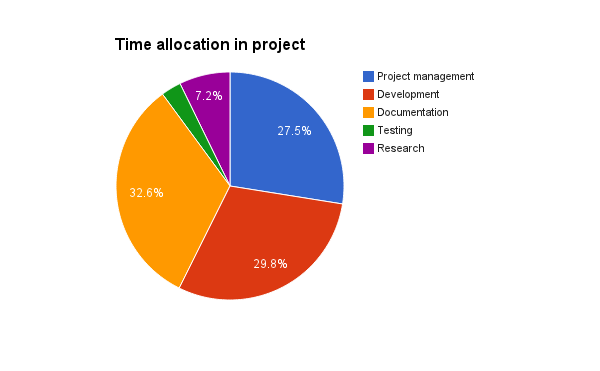
\includegraphics[width=0.6\textwidth, clip, trim=4cm 2cm 4cm 1cm]{ch/retrospect/fig/timePie.png}
\caption{Pie chart of time spent on different parts of the project}
\label{fig:piechart}
\end{figure}

When comparing the actual time spent with the estimated time from table~\ref{tab:timeEstWP}, it is clear that the team did not spend time in the manner that was estimated before the project started. The subsequent sections will comment on some of the deviations.

\begin{figure}[H]
\centering
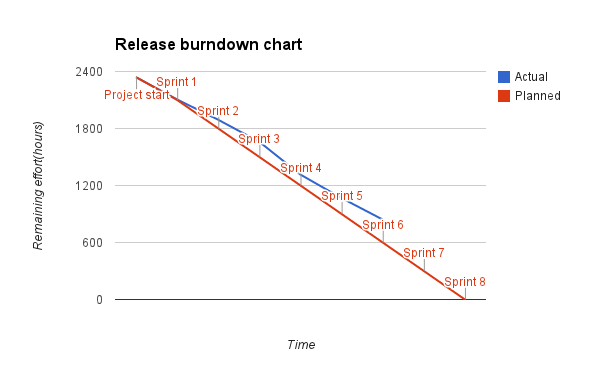
\includegraphics[width=0.7\textwidth, clip, trim=1.1cm 0.5cm 1.2cm 1cm]{ch/retrospect/fig/release.png}
\caption{Project release burn down chart}
\label{fig:release}
\end{figure}

\subsubsection{Deviations in testing}
One of the larger deviations is the estimated vs. logged effort is the time devoted to testing. The 2.8\% time logged for testing is more than three times lower than the 10\% that were estimated. This is because the time logged for testing is only time spent exclusively for testing. This includes user testing and acceptance testing, but not the functional testing which was done iteratively with development. Due to the way that the team ran functional tests, this time was logged as development instead of testing. We are therefore confident that we have spent closer to 10\% on testing and that the system is thoroughly tested.

\subsubsection{Deviations in project management}
The definitively largest abnormality lies in the project management that logged a total of 27.5\% of the spent time vs. the estimated 5\%. We believe that much of this is simply poor estimation done early in the project, but there are other factors that explain why this section is much higher than estimated. Project management consists mainly of hours logged for meetings. Many of the meetings had agendas that could classify it under either development or research. For example, the early prototyping of the user interface was done during prolonged meetings, and therefore logged as project management. In retrospect we should either have specified project management differently, or held meetings dedicated to development or research, and logged the time spent accordingly. As all our meeting were generic, it would be fruitless to try and categorize time spent in them. Even if these measures are taken, the team will estimate a higher percentage of time going towards project management in the future. 

\subsubsection{Comments on time spent}
In the release burn down chart, displayed in figure~\ref{fig:release}, the estimated project progress is compared with the progress that was actually made. As the graph shows, the team worked less than the estimated number of hours. After the end of sprint 8, the team had spent a total of 2084 hours since the beginning of sprint 1. This is 256 hours less than the 2340 hours the team planned to spend on the project.

There are several reasons for this, including unplanned absence of team members, underestimation of tasks and too heavy workload due to deliveries in other classes. Another factor in the discrepancy between the planned hours and the actual time spent is the manner of which work hours are logged. The hours logged in Yodiz, shown in figure~\ref{fig:release}, only represent how long specific tasks took to complete. The logging done in Yodiz is used primarily to estimate user stories and tasks, and not to log precise work hours. This gives a deviation in hours spent and hours logged, which in time amounts to a notable amount. 

The largest factor in the deviation however, was the change from 20 to 25 work hours per week as described in section~\ref{sec:availableHours}. If the team had not travelled to China, it would have had 9 sprints worth 240 hours each(20 hours person every week, as per course requirement) with a total of 2160 hours to spend on the project. The team's change to compensate for the trip to China left the team with 8 sprints worth 300 hours each, giving a total of 2340 working hours, as shown in table~\ref{tab:availHours}. This means that the team projected a usage of 180 hours more than the course requirement.

Considering the mentioned factors, we are happy with the effort we have laid down in this project. If one subtracts the 180 hours the team voluntarily added, only 76 work hours are missing from the expected effort for IT2901. We are confident that this 3\% discrepancy did not have much effect on the final product that we were able to deliver, and had it not been for the many preventative actions taken according to our risk analysis show in table~\ref{tab:risktable}, this percentage could have been a lot higher.

\subsection{Resource allocation}
As described in section~\ref{sec:availResources}, the team had several resources available, including a supervisor, and the customer. The team had internal meetings at least two times a week, and also an eight hour work session once a week. In addition, weekly meetings with the customer and meetings with the supervisor every other week were held.

To have meetings on such a regular basis has been of great value for the team. It saved a lot of time to have pre-booked meeting rooms, and it was also easier for the other parties involved in the project to prepare for the meetings.

During the meetings with the supervisor, the team were given valuable input and feedback regarding customer relations, and the content and structure of the report. Although the role of the supervisor was unclear to the team in the early stages of the project. It was quickly learned that he was more a guide the team could use for help, and not a supervisor that was in place to make sure work was being done. The only real oversight the supervisor had was the activity report which included a work log and a summary of the progress made since the last meeting.

Communicating with the customer on a regular basis reduced the probability of misunderstandings to arise and increased the likelihood that the team would deliver a product the customer would be greatly satisfied with. 

One of the most valuable decisions that was made in this project was to actually have fixed meeting times. This assured that the entire team was kept updated and involved. On these internal meetings, the team planned and distributed tasks among the team members, and discussed occurring issues. Each team member was assigned an area of responsibility, so that no important parts of the project would be neglected. It also turned out to be a way to keep the motivation high and further involve the team members.
